\documentclass[border=3pt]{standalone}
\usepackage{tikz}
\usetikzlibrary{arrows.meta,calc,positioning}
\tikzset{pin/.style={-{Stealth[length=5pt]}},
  blk/.style={draw, thick, font=\sffamily\small, align=center}}
\begin{document}
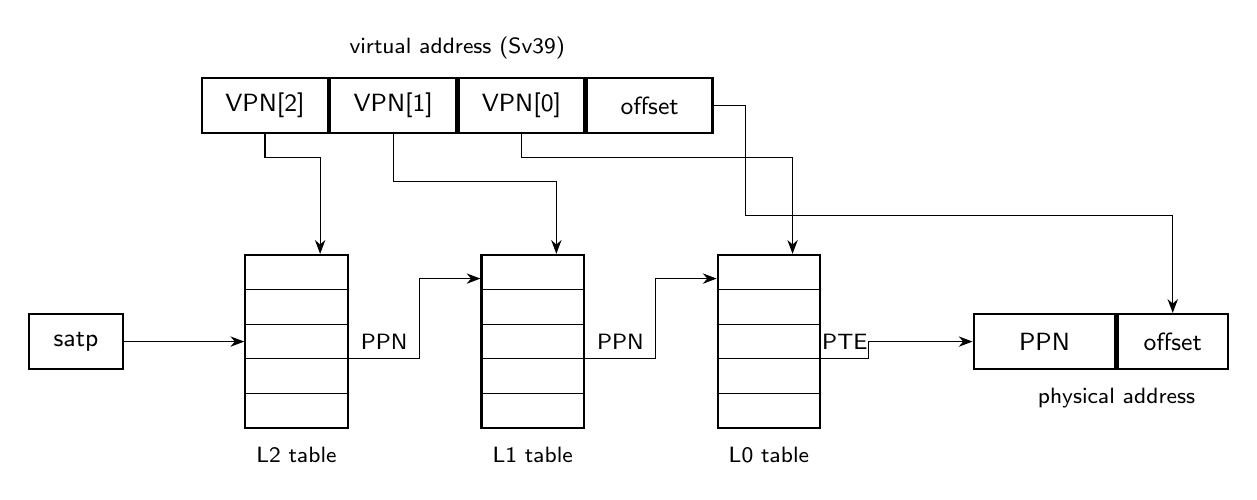
\begin{tikzpicture}[font=\sffamily\small]
  % VA fields
  \node[blk, minimum width=16mm, minimum height=7mm] (v2) at (0,0) {VPN[2]};
  \node[blk, minimum width=16mm, minimum height=7mm, anchor=west] (v1) at (v2.east) {VPN[1]};
  \node[blk, minimum width=16mm, minimum height=7mm, anchor=west] (v0) at (v1.east) {VPN[0]};
  \node[blk, minimum width=16mm, minimum height=7mm, anchor=west] (off) at (v0.east) {offset};
  \node[font=\sffamily\footnotesize, above=1mm of v1.north east] {virtual address (Sv39)};
  % page tables
  \node[blk, minimum width=13mm, minimum height=22mm] (pt2) at (0.4,-3.0) {};
  \node[blk, minimum width=13mm, minimum height=22mm] (pt1) at (3.4,-3.0) {};
  \node[blk, minimum width=13mm, minimum height=22mm] (pt0) at (6.4,-3.0) {};
  \foreach \n in {pt2,pt1,pt0}{\foreach \y in {-6.6,-2.2,2.2,6.6}{
    \draw ($(\n.west)+(0,\y mm)$) -- ($(\n.east)+(0,\y mm)$);}}
  \node[font=\sffamily\footnotesize, below=1mm of pt2.south] {L2 table};
  \node[font=\sffamily\footnotesize, below=1mm of pt1.south] {L1 table};
  \node[font=\sffamily\footnotesize, below=1mm of pt0.south] {L0 table};
  % satp
  \node[blk, minimum width=12mm, minimum height=7mm] (satp) at (-2.4,-3.0) {satp};
  \draw[pin] (satp.east) -- (pt2.west);
  % walk: each VPN indexes, entry points to next table base
  \draw[pin] (v2.south) -- ++(0,-3mm) -| ($(pt2.north)+(3mm,0)$);
  \draw[pin] ($(pt2.east)+(0,2.2mm-4.4mm)$) -- node[above, font=\sffamily\footnotesize]{PPN} ++(9mm,0) |- ($(pt1.west)+(0,8mm)$);
  \draw[pin] (v1.south) -- ++(0,-6mm) -| ($(pt1.north)+(3mm,0)$);
  \draw[pin] ($(pt1.east)+(0,-2.2mm)$) -- node[above, font=\sffamily\footnotesize]{PPN} ++(9mm,0) |- ($(pt0.west)+(0,8mm)$);
  \draw[pin] (v0.south) -- ++(0,-3mm) -| ($(pt0.north)+(3mm,0)$);
  % leaf PTE -> physical address
  \node[blk, minimum width=18mm, minimum height=7mm] (ppn) at (9.9,-3.0) {PPN};
  \node[blk, minimum width=14mm, minimum height=7mm, anchor=west] (poff) at (ppn.east) {offset};
  \node[font=\sffamily\footnotesize, below=1mm of ppn.south east] {physical address};
  \draw[pin] ($(pt0.east)+(0,-2.2mm)$) -- node[above, font=\sffamily\footnotesize]{PTE} ++(6mm,0) |- (ppn.west);
  \draw[pin] (off.east) -- ++(4mm,0) |- ++(0,-14mm) -| (poff.north);
\end{tikzpicture}
\end{document}
